In order to test the resulting solution we have implemented the frontend as a plugin using ReSharper~SDK\footnote{ReSharper developer's guide: \url{https://www.jetbrains.com/help/resharper/sdk/README.html}. Access Date: 15.08.2019}, so it can be installed into ReSharper\footnote{ReSharper: \url{https://www.jetbrains.com/resharper/}. Access Date: 15.08.2019}, Rider\footnote{Rider IDE: \url{https://www.jetbrains.com/rider/}. Access Date: 15.08.2019} and InspectCode\footnote{InspectCode tool: \url{https://www.jetbrains.com/help/resharper/InspectCode.html}. Access Date: 15.08.2019}.
The source code is parsed by internal ReSharper tools and the result is used to produce graphs and meta-information.
The issues found by the backend are shown using code highlighting.

The sample analysis which has been implemented is the taint tracking analysis.
It is defined by the PDA constructed in section 2.
We slightly modified it to better process interactions with object fields.
We accompany code highlighting with the complete path of a tainted variable from a source to a sink as a sequence of operatoins.
In ReSharper this information is shown when mouse is hovering over the problematic code.

\subsection{Taint analysis sample cases}

The resulting solution has been tested on a few common cases which can be found in the repository\footnote{Test cases: \url{github.com/gsvgit/CoFRA/tree/master/test/data/TaintAnalysis}}.
We demonstrate the principal properties of the analyzer with three of them.
We illustrate the examples with screenshots of the Rider IDE.
We relocated the tool-tips to not cover the source code.

The first feature is ensuring flow sensitivity.
This means that when the flow of variables being passed into and returned from the method is processed, we distinguish between different call sites and returns are done to the appropriate return points.
This is shown in fig~\ref{fig:ReturnsAndBrackets}.
This example illustrates the most common cases of interprocedural data passing.
\textit{Brackets} method gets the data, possibly performs some computations on them and returns the result.
Invocations at lines 37 and 38 show that the solution can distinguish two data flow paths despite both of them passes through the same method.
So, \textit{e} becomes tainted because \textit{c} is tainted and \textit{f} does not because \textit{d} is clear.
%Moreover, the analyzer can track paths where passes and returns do not form the correct bracket sequence that is shown by method \textit{PostSource} which does not take any parameter and just returns tainted data.

\begin{figure}[h]
    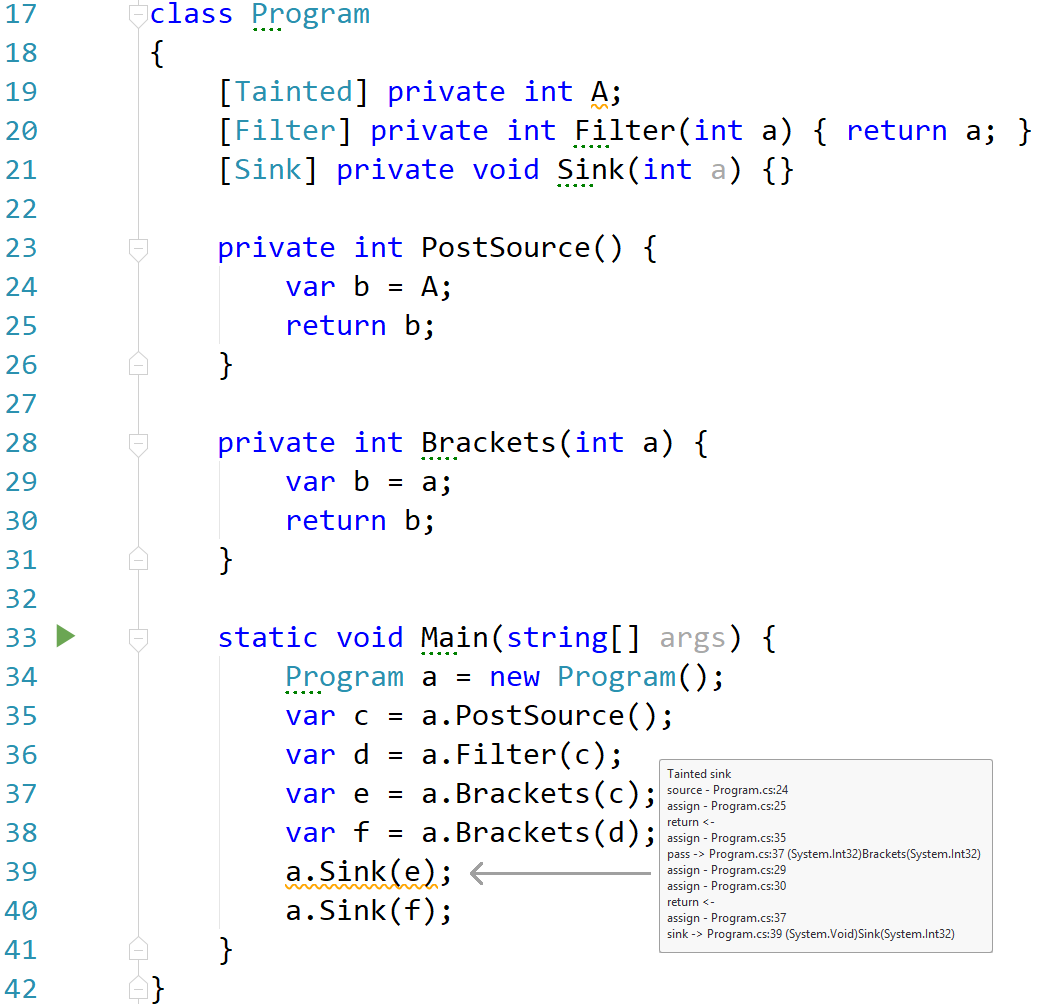
\includegraphics[width=\linewidth]{screenshots/ReturnsAndBrackets.png}
    \caption{Flow sensitivity}
    \label{fig:ReturnsAndBrackets}
\end{figure}

The second feature is context sensitivity.
Context sensitivity is necessary to track the propagation of objects that are tainted by assigning of some fields inside them both by their own methods and by outer code interacting with their fields directly.
However, it is impossible to provide true context-sensitivity since it cannot be expressed alongside with flow-sensitivity~\cite{Spath:2019:CFF:3302515.3290361}.
As a result, in our analysis we provide a limited context sensitivity, which is shown in fig~\ref{fig:ObjectTainting}.
There is the field \textit{B} in line 18.
This field can be used widely in the logic of the \textit{Container} class and by this, the tainting of this field is considered as the tainting of the whole object.
However, while processing of the method \textit{Store} during the analysis it is hard to decide what the object needs to be tainted because in the inner context of \textit{Store} it is just \textit{this} object.
We must consider the calling context to make such decision.
The solution provides this opportunity which is illustrated by lines 33-36 where the first invocation of \textit{Store} leads to the tainting of object \textit{d} and the second invocation does not taint object \textit{e}.

\begin{figure}[h]
    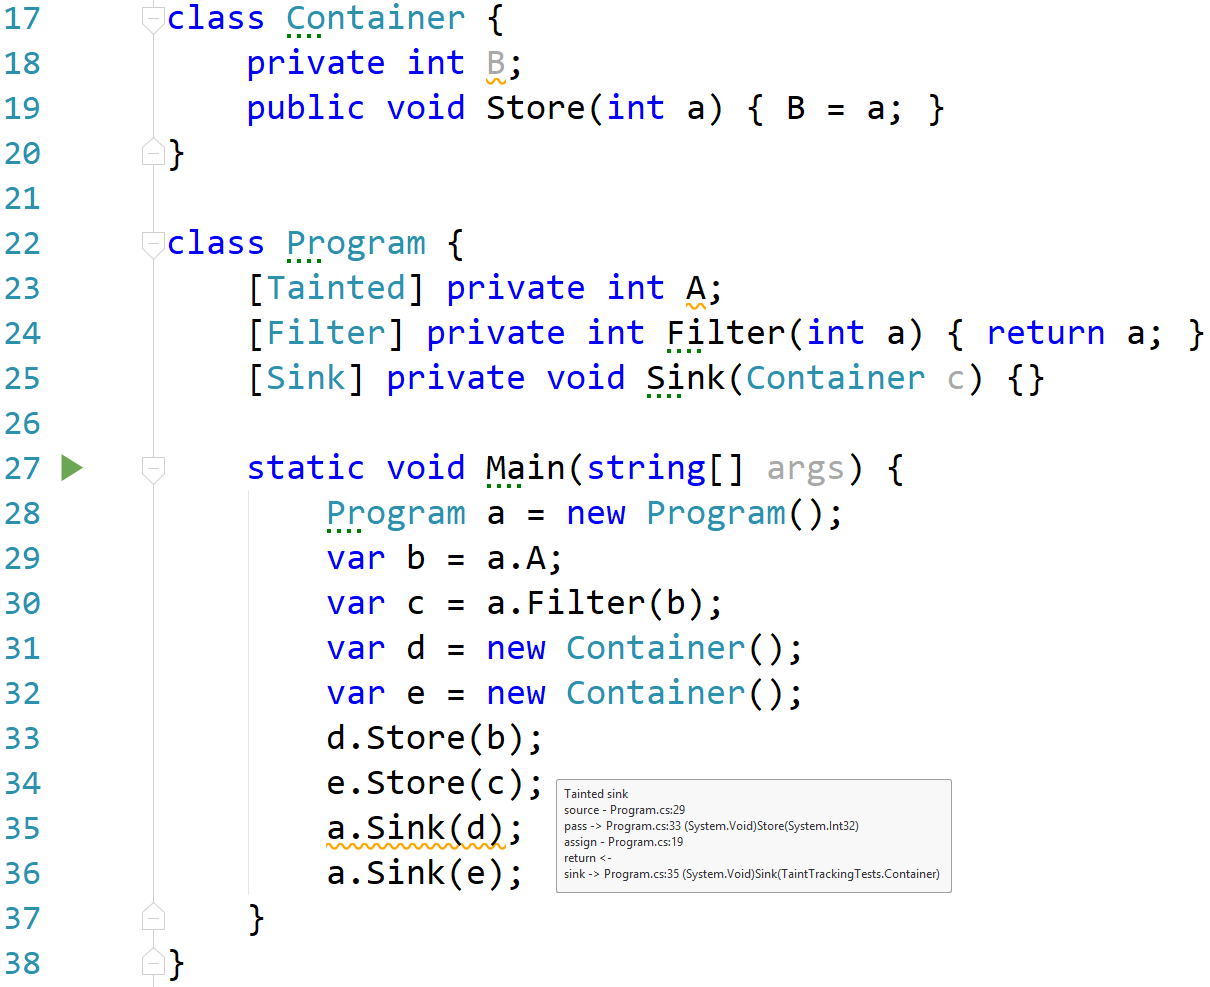
\includegraphics[width=\linewidth]{screenshots/ContextSensitivity.png}
    \caption{Tainting of an object by its own method}
    \label{fig:ObjectTainting}
\end{figure}

Finally, the solution works with any type of recursion and does not fall into infinite cycles.
This case is demonstrated in fig.~\ref{fig:Recursion}.
This snippet contains two mutually recursive methods which pass the data to each other.
The solution checks all possible paths of passing including those with cyclic invocations and returns the passed variable to the point corresponding to the initial invocation.

\begin{figure}[h]
    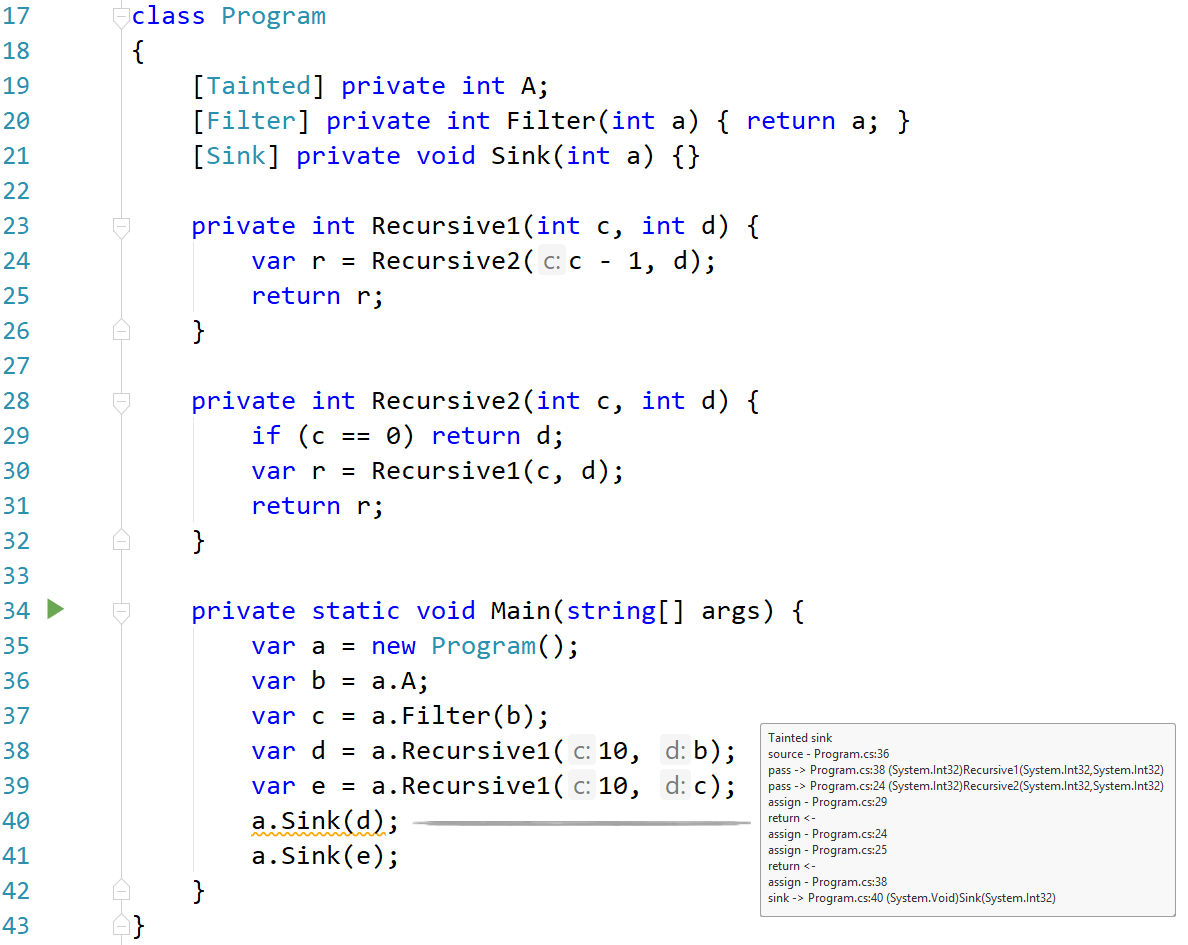
\includegraphics[width=\linewidth]{screenshots/Recursion.png}
    \caption{Recursive methods processing}
    \label{fig:Recursion}
\end{figure}

\subsection{Performance}

It is also necessary to measure the performance of the resulting solution.
To measure performance we could have used the taint analysis, but it requires to equip all points of interest by corresponded attributes manually.
Considering this, we decided to instead implement a different kind of analysis which tracks the propagation of all variables and by this explores any possible path in the graph.
Thus, the time and space required for its execution should be a consistent estimation of the efficiency of the solution.

The code base which has been chosen as a source of data is the full solutions of a few big projects: Mono\footnote{Source code of mono project: \url{https://github.com/mono/mono}. Access Date: 15.08.2019}, EventStore\footnote{Source code of EventStore project: \url{https://github.com/EventStore/EventStore}. Access Date: 15.08.2019} and OpenRA\footnote{Source code of OpenRA project: \url{https://github.com/OpenRA/OpenRA}. Access Date: 15.08.2019}.
The analyzer has been tested on a computer running Windows~10 with quad-core Intel Core i7 3.4 GHz CPU and 16 GB of RAM.
The results are shown in the table~\ref{tab:Performance}.
Execution time does not include the time required for graph construction.

\begin{table}[h]
    \begin{tabular}{|l|l|l|l|l|}
    \hline
        Project & Classes & Methods & \begin{tabular}[c]{@{}l@{}}Execution \\ time (s)\end{tabular} & \begin{tabular}[c]{@{}l@{}}Allocated \\ memory \\ (GB)\end{tabular} \\ \hline
            Mono & 21013 & 192745 & $21\pm 0.5$ & $\sim 4.2$ \\ \hline
        EventStore & 3828 & 22796 & $2.7\pm 0.1$ & $\sim 0.49$ \\ \hline
        OpenRA & 2767 & 15451 & $2.3\pm 0.1$ & $\sim 0.4$ \\ \hline
    \end{tabular}
    \caption{Performance}
    \label{tab:Performance}
\end{table}

We conclude that our solution is able to process real-world projects in acceptable time.
